%%%%%%%%%%%%%%%%%%%%%%%%%%%%%%%%%%%%%%%%%
% Beamer Presentation
% LaTeX Template
% Version 1.0 (10/11/12)
%
% This template has been downloaded from:
% http://www.LaTeXTemplates.com
%
% License:
% CC BY-NC-SA 3.0 (http://creativecommons.org/licenses/by-nc-sa/3.0/)
%
%%%%%%%%%%%%%%%%%%%%%%%%%%%%%%%%%%%%%%%%%

%----------------------------------------------------------------------------------------
%	PACKAGES AND THEMES
%----------------------------------------------------------------------------------------

\documentclass{beamer}

\mode<presentation> {

% The Beamer class comes with a number of default slide themes
% which change the colors and layouts of slides. Below this is a list
% of all the themes, uncomment each in turn to see what they look like.

%\usetheme{default}
%\usetheme{AnnArbor}
%\usetheme{Antibes}
%\usetheme{Bergen}
%\usetheme{Berkeley} %with Outline
%\usetheme{Berlin}
%\usetheme{Boadilla}
\usetheme{CambridgeUS} %This is well-looking
%\usetheme{Copenhagen}
%\usetheme{Darmstadt}
%\usetheme{Dresden}
%\usetheme{Frankfurt}
%\usetheme{Goettingen}
%\usetheme{Hannover}
%\usetheme{Ilmenau}
%\usetheme{JuanLesPins}
%\usetheme{Luebeck}
%\usetheme{Madrid}
%\usetheme{Malmoe}
%\usetheme{Marburg}
%\usetheme{Montpellier}
%\usetheme{PaloAlto}
%\usetheme{Pittsburgh}
%\usetheme{Rochester}
%\usetheme{Singapore}
%\usetheme{Szeged}
%\usetheme{Warsaw}

% As well as themes, the Beamer class has a number of color themes
% for any slide theme. Uncomment each of these in turn to see how it
% changes the colors of your current slide theme.

%\usecolortheme{albatross}
%\usecolortheme{beaver}
%\usecolortheme{beetle}
%\usecolortheme{crane}
\usecolortheme{dolphin}
%\usecolortheme{dove}
%\usecolortheme{fly}
%\usecolortheme{lily}
%\usecolortheme{orchid}
%\usecolortheme{rose}
%\usecolortheme{seagull}
%\usecolortheme{seahorse}
%\usecolortheme{whale}
%\usecolortheme{wolverine}

%\setbeamertemplate{footline} % To remove the footer line in all slides uncomment this line
%\setbeamertemplate{footline}[page number] % To replace the footer line in all slides with a simple slide count uncomment this line

%\setbeamertemplate{navigation symbols}{} % To remove the navigation symbols from the bottom of all slides uncomment this line
}

\usepackage{graphicx} % Allows including images
\usepackage{booktabs} % Allows the use of \toprule, \midrule and \bottomrule in tables
\usepackage{amsmath, amssymb, amsfonts}
\usepackage{mathrsfs}
\usepackage{amsthm}
%----------------------------------------------------------------------------------------
%	TITLE PAGE
%----------------------------------------------------------------------------------------

\title[VE216]{VE216 Recitation Class 9} % The short title appears at the bottom of every slide, the full title is only on the title page

\author{ZHU Yilun} % Your name
\institute[SJTU] % Your institution as it will appear on the bottom of every slide, may be shorthand to save space
{
UM-SJTU Joint Institute \\ % Your institution for the title page
\medskip
\textit{VE216 SU20 TA Group} % Your email address
}
\date{2020 Summer} % Date, can be changed to a custom date e.g.:\today

\begin{document}

\begin{frame}
\titlepage % Print the title page as the first slide
\end{frame}

\begin{frame}
\frametitle{Overview} % Table of contents slide, comment this block out to remove it
\tableofcontents % Throughout your presentation, if you choose to use \section{} and \subsection{} commands, these will automatically be printed on this slide as an overview of your presentation
\end{frame}

%----------------------------------------------------------------------------------------
%	PRESENTATION SLIDES
%----------------------------------------------------------------------------------------






%-------------------------------------------------
\section{Chapter 8: Communications}
%--------------------------------------------------
\subsection{Sinusoidal Amplitude Modulation (AM) - Synchronous}

\begin{frame}
\frametitle{Modulation}
\begin{itemize}
\item Modulation Property:
\begin{figure}
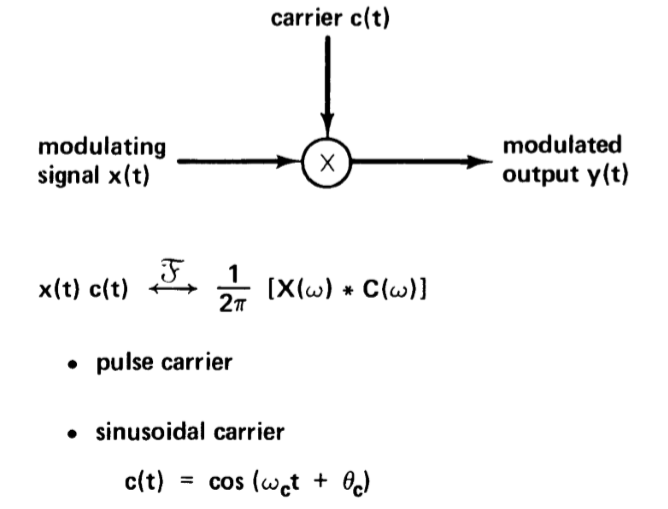
\includegraphics[width=0.8\linewidth]{AM1}
\end{figure}
\end{itemize}
\end{frame}

\begin{frame}
\frametitle{Sinusoidal Amplitude Modulation}
\begin{itemize}
\item Block diagram of modulation system: \\
$x(t)$ - information, $c(t)$ - carrier
\begin{figure}
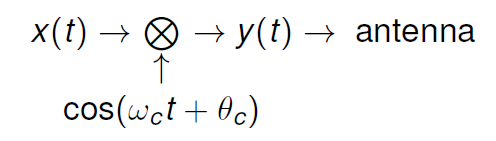
\includegraphics[width=0.5\linewidth]{AM2}
\end{figure}
Notice: here we multiply the carrier signal rather than do convolution
\item Transmitted signal (i.e., modulated output $y(t)$):
\begin{figure}
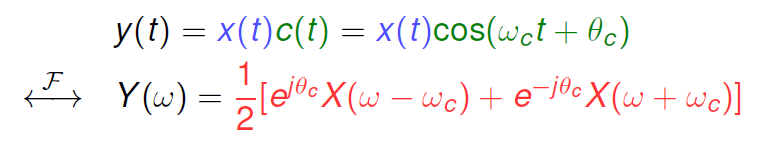
\includegraphics[width=0.7\linewidth]{AM3}
\end{figure}
\end{itemize}
\end{frame}

\begin{frame}
\frametitle{Sinusoidal Amplitude Modulation - Synchronous}
\begin{figure}
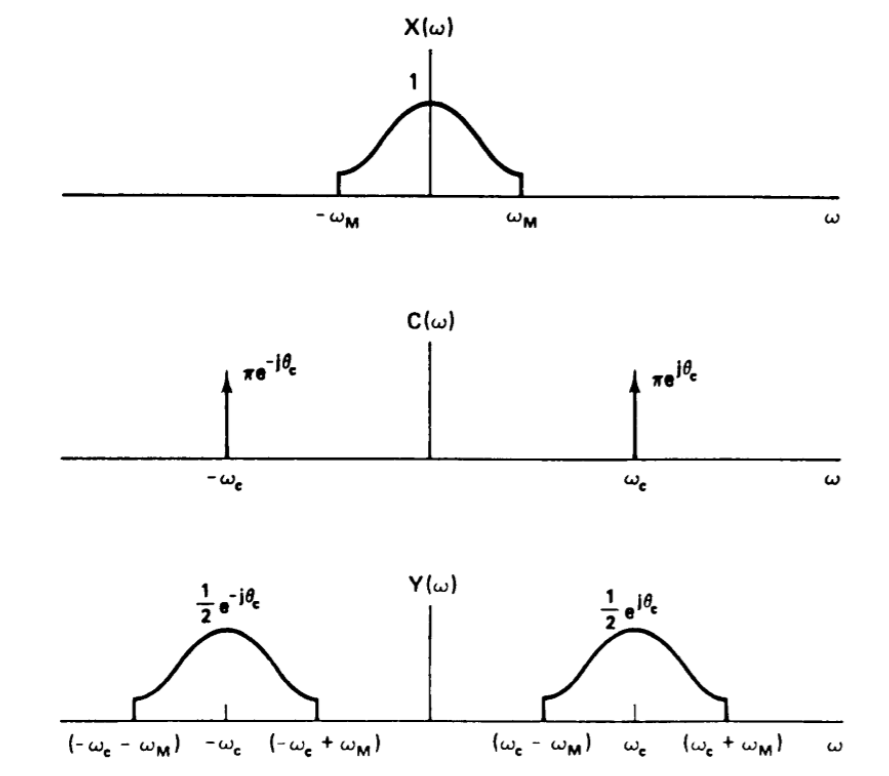
\includegraphics[width=0.7\linewidth]{AM4}
\end{figure}
\end{frame}


\begin{frame}
\frametitle{Synchronous Demodulation}
\begin{itemize}
\item Block diagram of demodulation system:
\begin{figure}
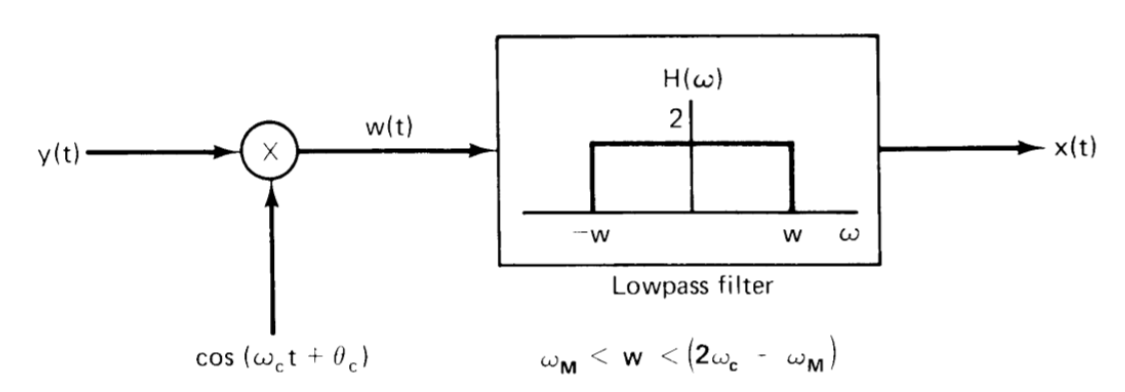
\includegraphics[width=0.7\linewidth]{demod1}
\end{figure}
\item First multiply $y(t)$ by another $cos(\omega_ct + \theta_c)$ signal:
\begin{figure}
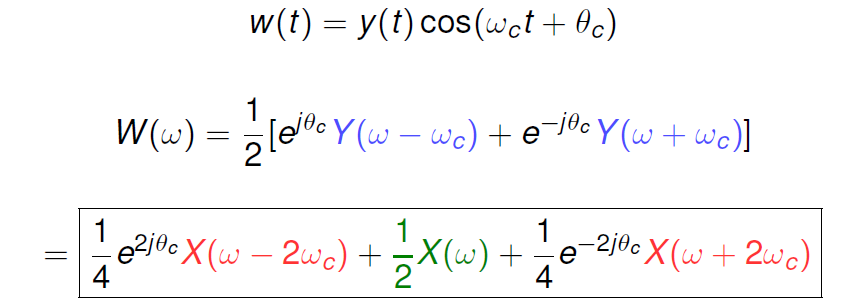
\includegraphics[width=0.6\linewidth]{demod2}
\end{figure}
\item Then followed by lowpass filtering to extract $ X(\omega)$
\end{itemize}
\end{frame}

\begin{frame}
\frametitle{Synchronous Demodulation}
\begin{figure}
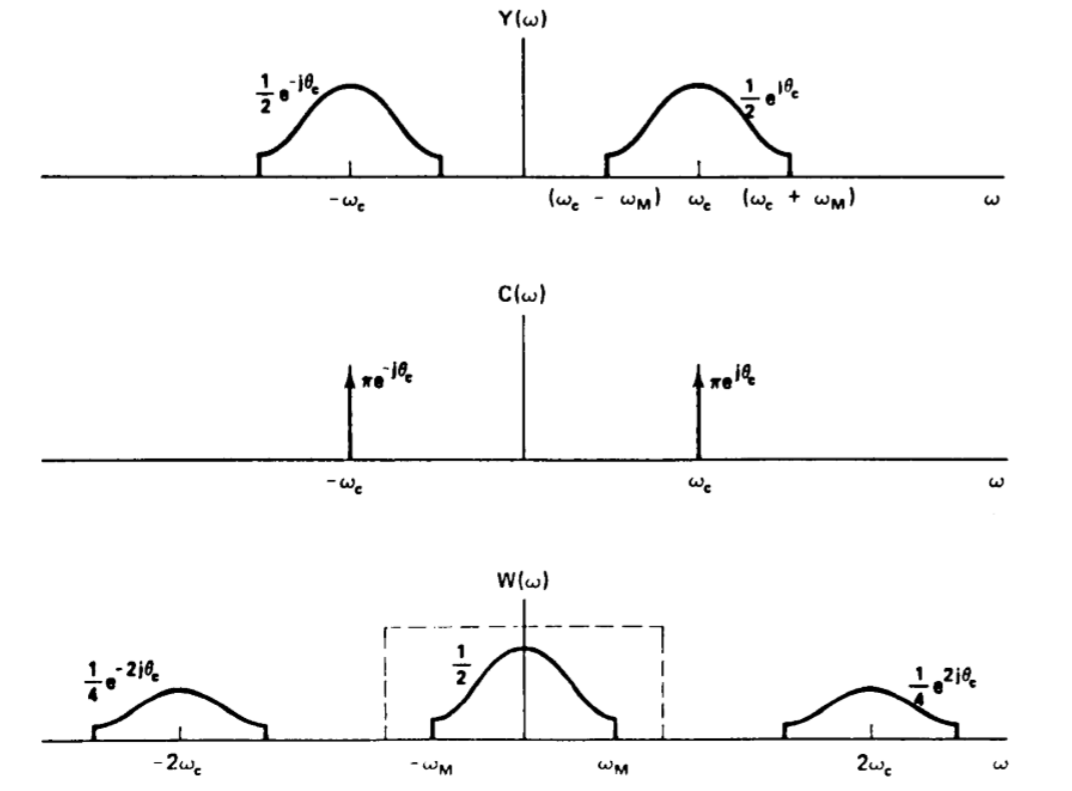
\includegraphics[width=0.8\linewidth]{demod3}
\end{figure}
\end{frame}


\subsection{Sinusoidal Amplitude Modulation (AM) - Asynchronous}
\begin{frame}
\frametitle{Asynchronous Demodulation: Motivation}
\begin{itemize}
\item It seems to be harmless to write the way synchronous Demodulation works on paper, but up to now we haven't considered how to implement it to hardware.
\item The bad news is that in practice, it is possible that both the frequency $\omega_c$ the phase $\theta_c$ are not available, therefore may need a sophisticated receiver
\item But for commercial products like AM radio, one would expect the receivers to be simple and inexpensive. 
\item Therefore a different demodulation scheme is needed, which uses a more complicated and power inefficient transmitter, but a simple receiver.
\end{itemize}
\end{frame}

\begin{frame}
\frametitle{Asynchronous Demodulation: Modulated signal}
\begin{itemize}
\item Now the modulated signal is: $y(t) = (A + x(t))\cos(\omega_ct)$
\item Often we choose $A$ greater then the amplitude of $x(t)$
\item The block diagram $\&$ how the output $y(t)$ looks like:
\begin{figure}
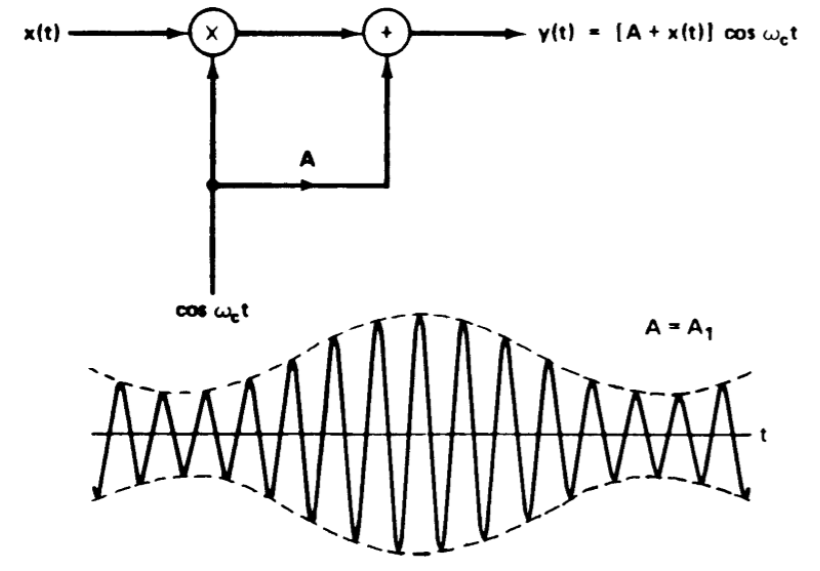
\includegraphics[width=0.6\linewidth]{asyn2}
\end{figure}
\end{itemize}
\end{frame}

\begin{frame}
\frametitle{Asynchronous Demodulation: Frequency Domain}
\begin{itemize}
\item In frequency domain: 
\begin{figure}
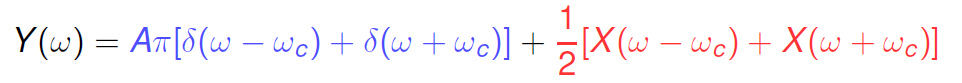
\includegraphics[width=0.8\linewidth]{asyn1}
\end{figure}
\begin{figure}
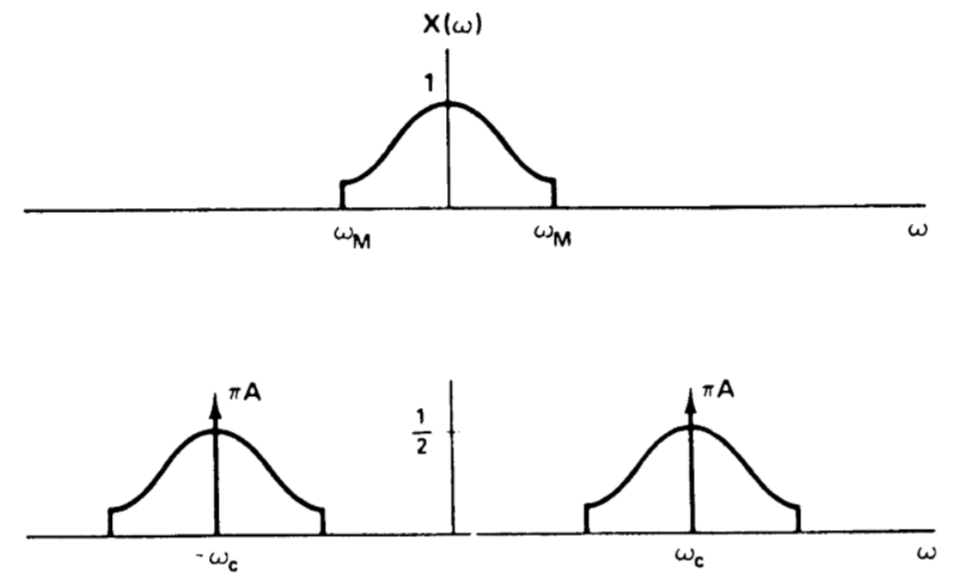
\includegraphics[width=0.8\linewidth]{asyn3}
\end{figure}
\end{itemize} 
\end{frame}

\begin{frame}
\frametitle{Asynchronous Demodulation}
\begin{itemize}
\item Use a simple circuit to detect the envelop: $m(t) = A + \hat{x}(t)$
\item It works because  $\omega_c$ is much higher than frequency of $x(t)$
\begin{figure}
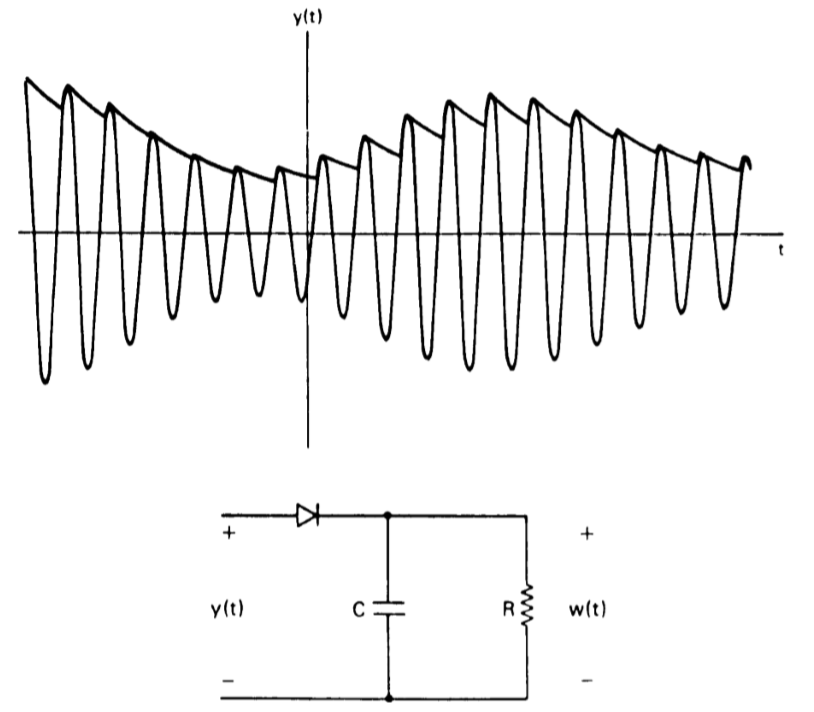
\includegraphics[width=0.6\linewidth]{asyn4}
\end{figure}
\end{itemize}
\end{frame}

\begin{frame}
\frametitle{Asynchronous Demodulation}
\begin{itemize}
\item The envolope detector gives us:
\begin{figure}
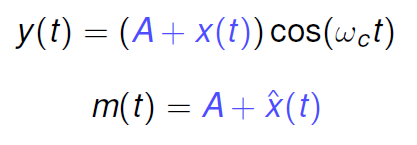
\includegraphics[width=0.4\linewidth]{asyn6}
\end{figure}
\item Then eliminate the DC component (this is what we mean by ``power inefficient'') and you recover the orginal signal.
\item The overall block diagram of demodulation:
\begin{figure}
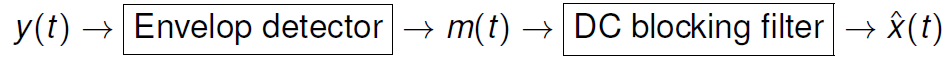
\includegraphics[width=0.8\linewidth]{asyn5}
\end{figure}
\end{itemize}
\end{frame}

\subsection{Frequency-division Multiplexing}
\begin{frame}
\frametitle{Frequency-division Multiplexing}
In time domain:
\begin{figure}
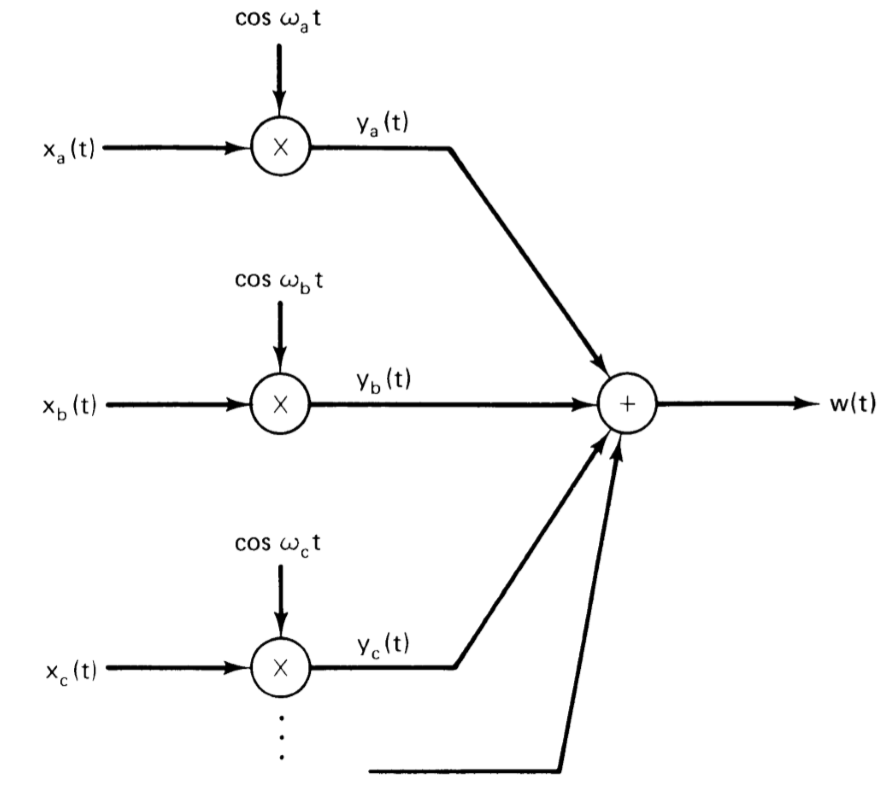
\includegraphics[width=0.6\linewidth]{multi1}
\end{figure}
\end{frame}

\begin{frame}
\frametitle{Frequency-division Multiplexing}
In frequency domain:
\begin{figure}
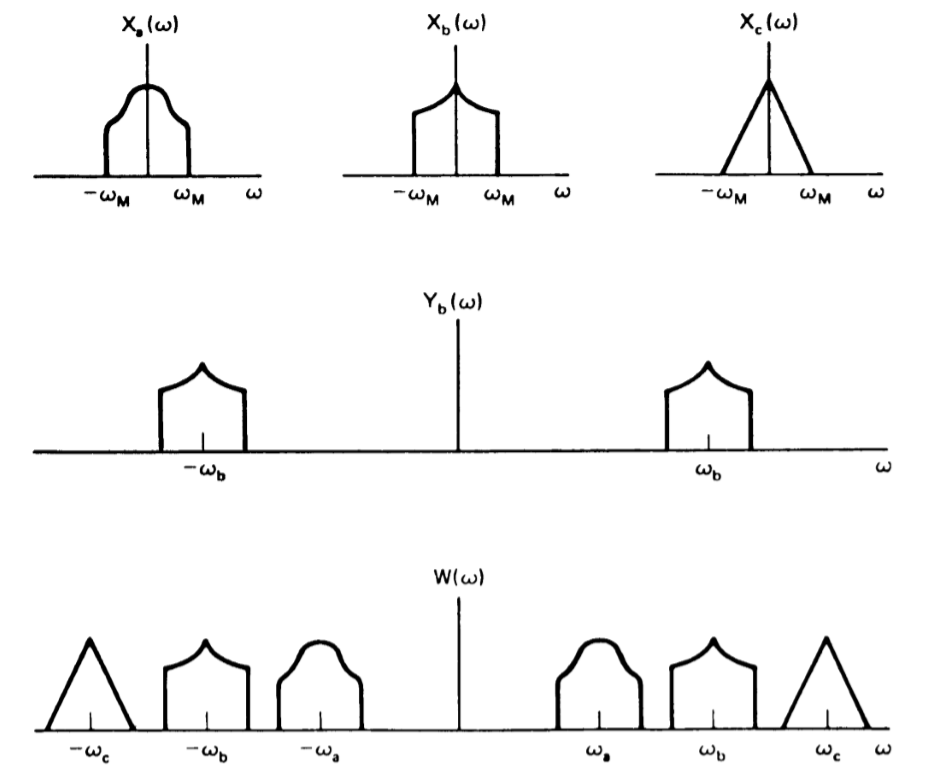
\includegraphics[width=0.6\linewidth]{multi2}
\end{figure}
\end{frame}

\begin{frame}
\frametitle{Demultiplexing and Demodulation}
\begin{itemize}
\item synchronous demodulation
\begin{figure}
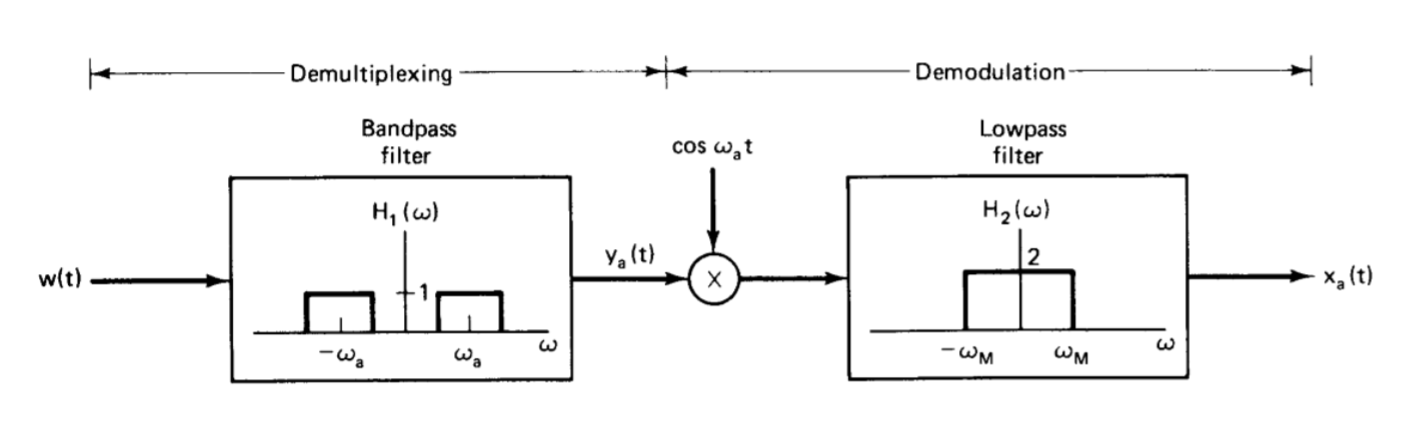
\includegraphics[width=0.7\linewidth]{multi3}
\end{figure}
\item asynchronous demodulation (using IF filter)
\begin{figure}
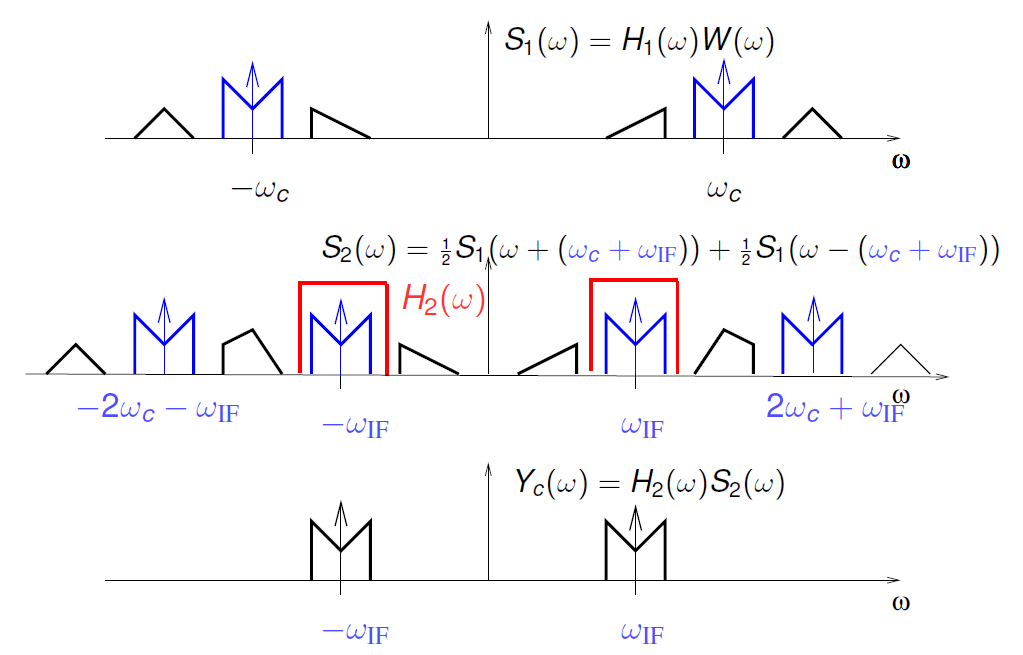
\includegraphics[width=0.5\linewidth]{multi4}
\end{figure}
\end{itemize}
\end{frame}

\begin{frame}[t]
    \frametitle{Exercise}
    \begin{figure}
        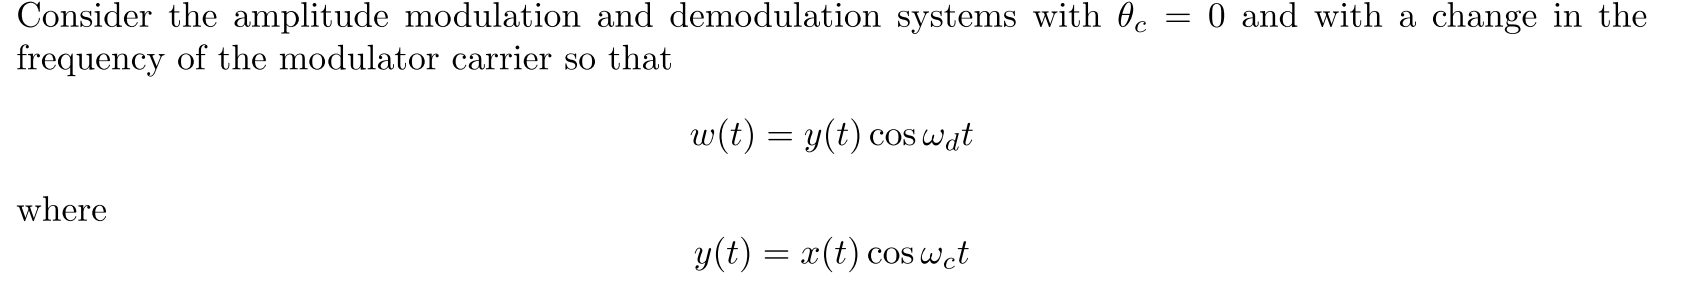
\includegraphics[width=0.8\linewidth]{q8a}
        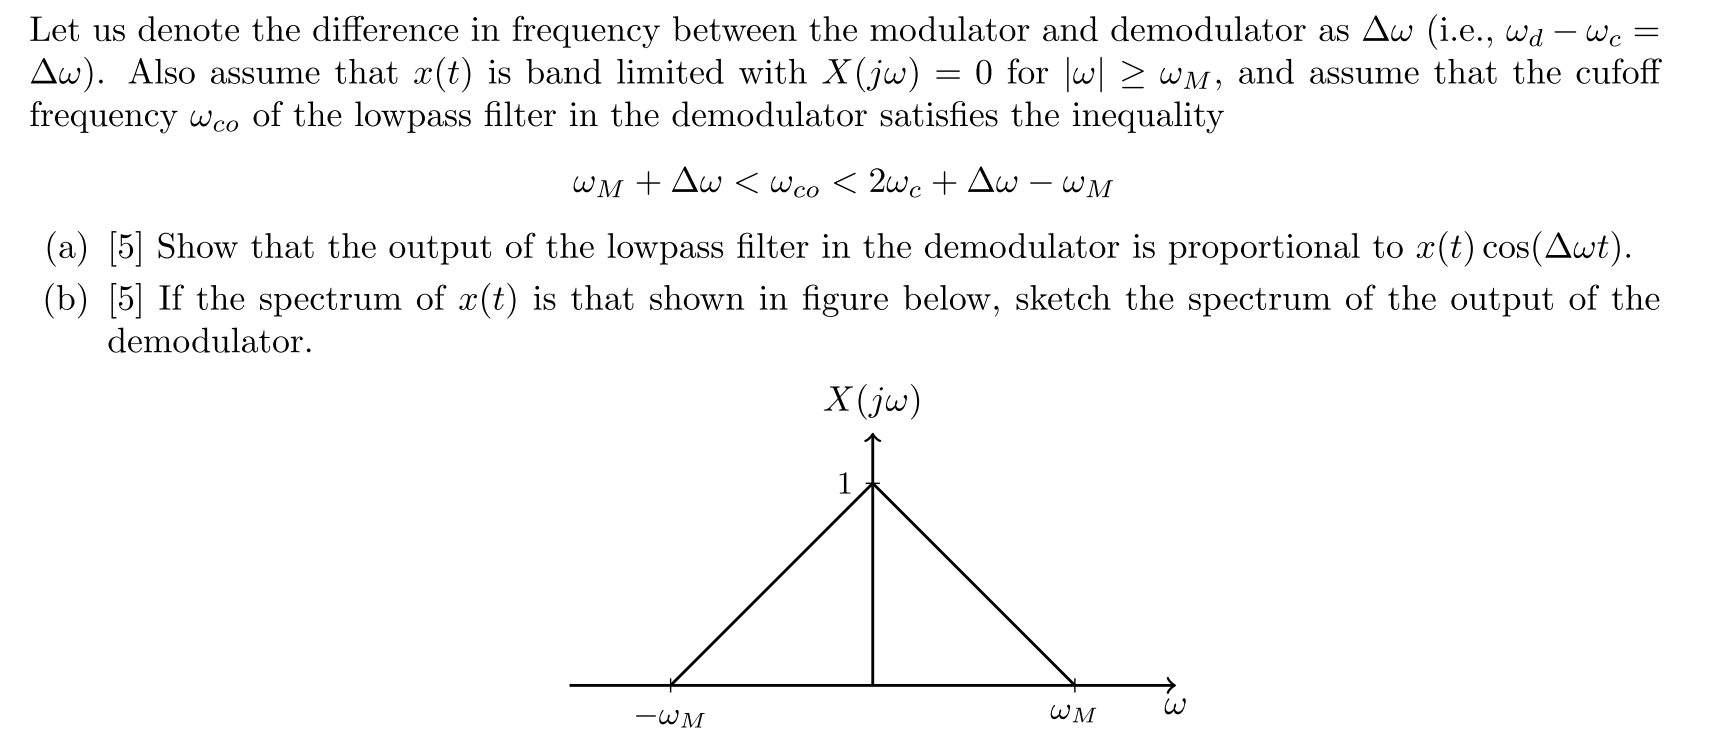
\includegraphics[width=0.8\linewidth]{q8b}
    \end{figure}

\end{frame}

\begin{frame}
    \frametitle{Lab2}
    \begin{itemize}
        \item I am completely lost when I first learnt Chap.8 Communication System, it was only after completing Prelab2 that I finally understood.
        \item Please take a close look at Prelab2 Section 2.3 - 2.6  
        \begin{figure}
            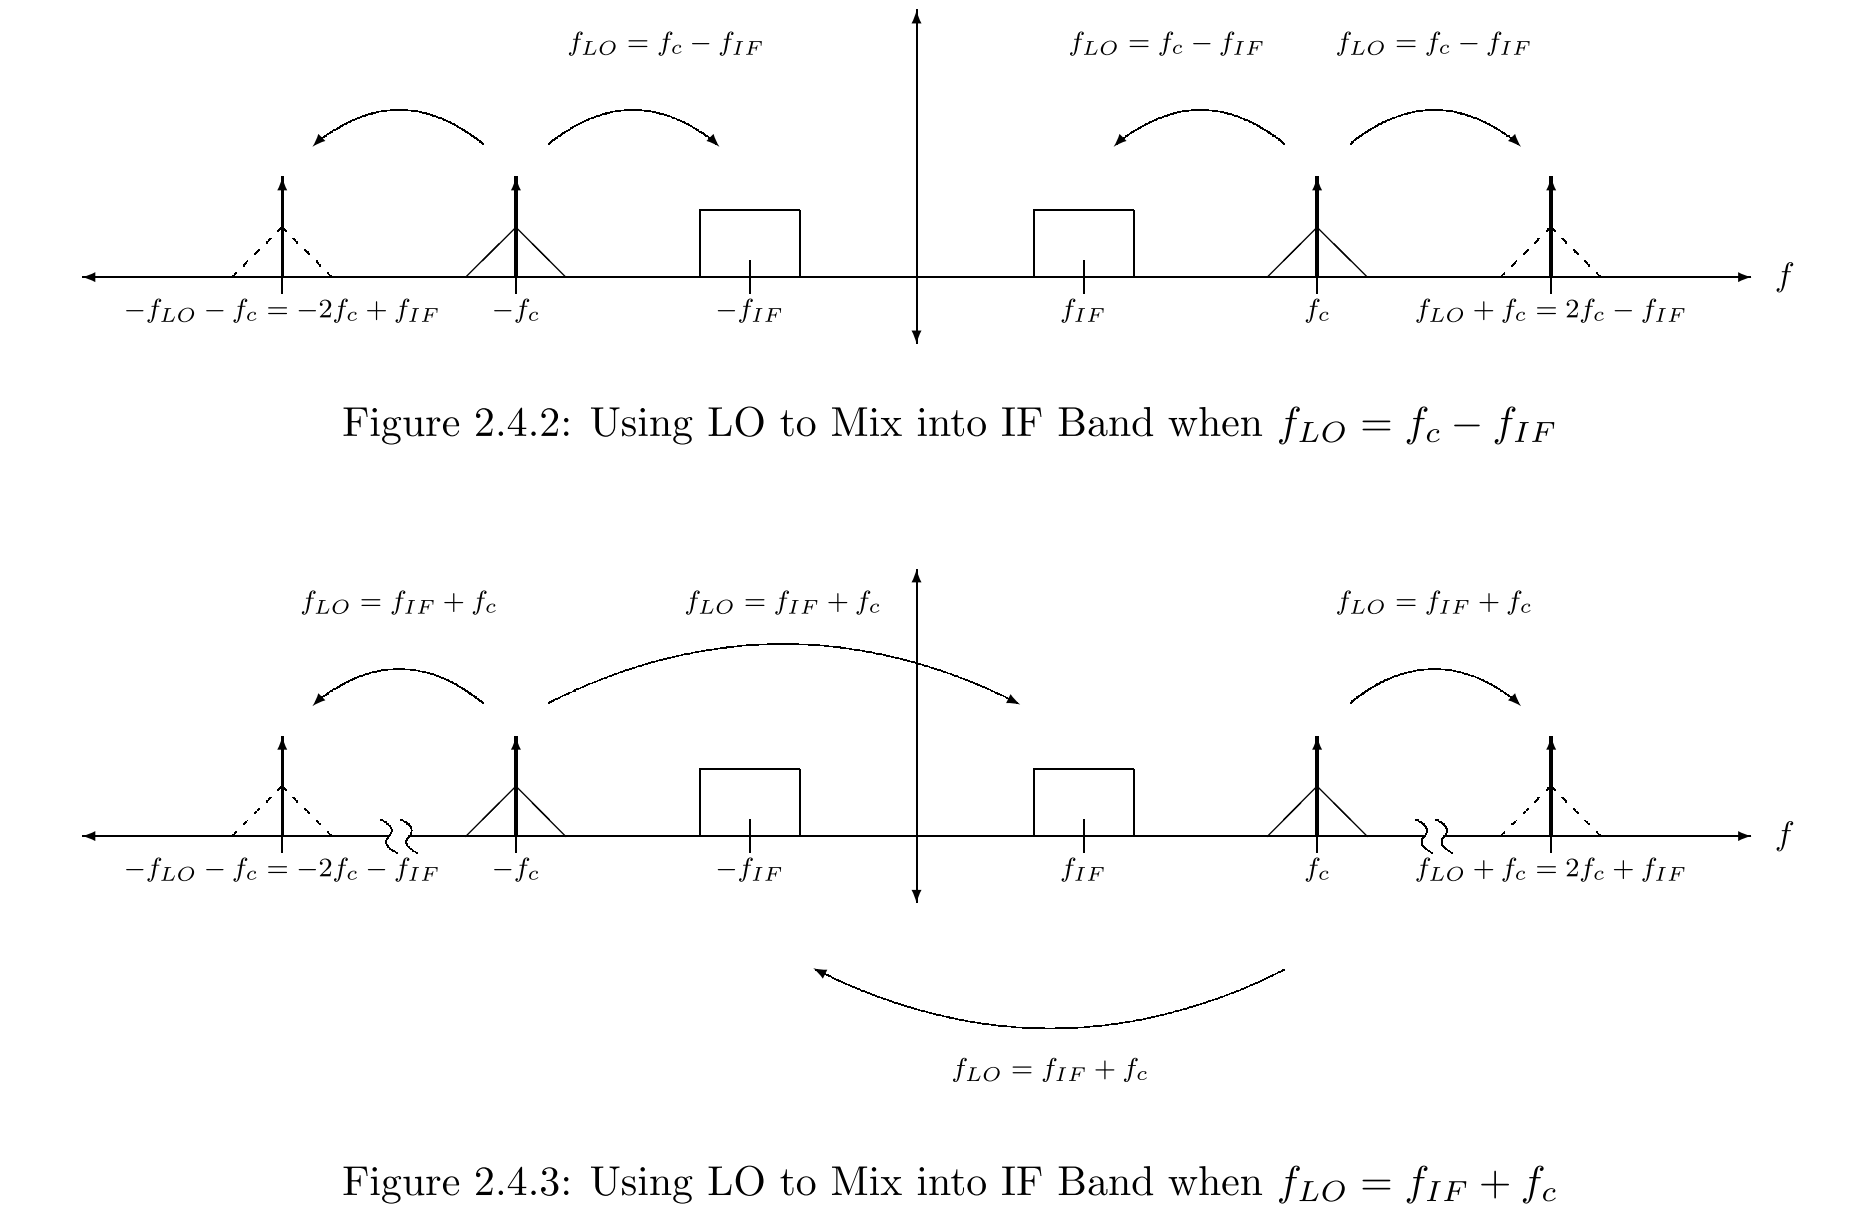
\includegraphics[width=0.6\linewidth]{prelab2.PNG}
        \end{figure}  
        \item Let's see a video on what really happens in real life - MIT Video Lecture 14 (30:10 – 33:00 min)
           
    \end{itemize}
    
\end{frame}


\section{Conclusion}
\begin{frame}
    \frametitle{Conclusion}
    \begin{itemize}
    \item Have a close look at Prelab2 and Quiz7, then you'll be the expert to Chap. 8
    \item Get the big picture of mod. \& demod.; solve problems graphically 
    \item I guess at one time you may complain about why do we have to go through such a painful way just to get $x(t)$. 
    \item But in fact the task is not at all easy, given the constrain of physical laws and hardware implementation.
    \item Using Asynchronous way (against syn.) is the first time in my collage life that I saw how the real life implementation affects our design 
    \item Therefore, to me, the outcomes of these issues are amazing, because Electrical Engineers not only managed to develop a brand new subject based on the fairly abstract mathematical property (associated with the Fourier transform), but also turn the theory into real life applications. 
     \end{itemize}
\end{frame}

%------------------------------------------------

\begin{frame}
\Huge{\centerline{The End}}
\end{frame}

%----------------------------------------------------------------------------------------

\end{document} 